Funktionen, die sich nach einem bestimmten Zeitraum $T$ oder einer bestimmten
Distanz $D$ wiederholen, werden periodische Funktionen genannt. Für diese muss
\begin{align}
  f(t + T) &= f(t) \\
  \text{bzw.}\quad f(x + D) &= f(x)
\end{align}
gelten. Die periodischen Funktionen die am häufigsten vorkommen sind die
Cosinus- und die Sinusfunktion. Diese lassen sich allgemein als
\begin{align}
  f(t) &= a\sin\biggl(\frac{2\pi}{T}\,t\biggr) \\
    \text{bzw.}\quad f(t) &= b\cos\biggl(\frac{2\pi}{T}\,t\biggr)
\end{align}
darstellen. Hierbei sind $a$ und $b$ die Aplituden und $T$ die jeweilige
Periodendauer. Fast alle der in der Natur vorkommenden periodischen Vorgänge
lassen sich mit diesen Funktionen darstellen.
\subsection{Das Fouriersche Theorem}
Laut dem Fourierschen Prinzip gilt
\begin{equation}
  f(t)=\frac{1}{2}a_0+\sum_{n=1}^\infty\biggl(a_\su{n}\cos\biggl(\frac{2\pi n}{T}t\biggr)
  +b_\su{n}\sin\biggl(\frac{2\pi n}{T}t\biggr)\biggr)
  \label{theorem} ,
\end{equation}
sofern die Reihe konvergiert. Die Koeffizienten $a_\su{n}$ und $b_\su{n}$
lassen sich über die Integrale
\begin{equation}
 \begin{split}
  a_\su{n} &= \frac{2}{T}\int\limits_{0}^{T} f(t)\cos\biggl(\frac{2\pi n}{T}t\biggr)dt \\
  \text{und}\quad b_\su{n} &= \frac{2}{T}\int\limits_{0}^{T} f(t)\sin\biggl(\frac{2\pi n}
  {T}t\biggr)dt
  \label{eq:analyse}
 \end{split}
\end{equation}
berechnen. In der Fourier-Entwicklung treten neben der Grundfrequenz
$\nu_1=\frac{1}{T}$ nur ganzzahlige Vielfache von $\nu_1$ auf. Diese werden auch
als harmonische Oberschwingungen bezeichnet. Zudem kommen in \eqref{theorem} nur
die Phasen $0, \frac{\pi}{2}, \pi$ und $\frac{3\pi}{2}$ vor.
Die Ermittlung der Amplituden nach \eqref{eq:analyse} bezeichnet man als
harmonische, beziehungsweise Fourier-Analyse.
\newpage
Wenn die Amplituden der
Teilschwingungen als Funktion der Frequenz dargestellt werden, so erhält man ein
Spektrum der Schwingung. Nach \eqref{theorem} muss dieses Spektrum ein
Linienspektrum sein, wie es in Abbildung \ref{spektrum} zu sehen ist.
\begin{figure}[H]
  \centering
  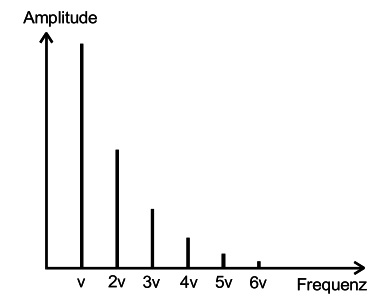
\includegraphics{bilder/linienspektrum.jpg}
  \caption{Linienspektrum einer periodischen Schwingung mit Grundfrequenz $\nu$
  \cite{351}}
  \label{spektrum}
\end{figure}
Desweiteren müssen die Amplituden $a_\su{n}$ und $b_\su{n}$ für
$n\rightarrow\infty$ gegen 0 gehen, da die Reihe nur dann konvergiert.
Wenn die geforderte Konvergenz nicht erfüllt ist, kann mit dem Fourierschen
Theorem die unstetige Stelle der Funktion nicht approximieren. In diesem Fall
tritt eine endliche Abweichung ein, die als Gibbsches Prinzip bezeichnet wird.
\subsection{Die Fourier-Transformation}
Mit Hilfe der Fourier-Transformation ist es möglich das gesamte Frequenzspektrum
der zeitabhängigen Funktion zu bestimmen. Hierbei spielt es keine Rolle, ob
$f$ periodisch ist, oder nicht. Die Fourier-Transformation hat die Form
\begin{equation}
  g(\nu) = \int\limits_{-\infty}^{\infty}f(t)\su{e}^{\su{i}\nu t},
\end{equation}
wobei $g(\nu)$ das Frequenzspektrum der Funktion darstellt. Ist $f$ periodisch,
besteht $g$ aus einer konvergierenden Reihe von $\delta$-Funktionen und man
erhält ein Linienspektrum, wie bereits in \ref{spektrum} zu sehen. Ist $f$
hingegen nicht periodisch, so erhält man ein kontinuierliches Frequenzspektrum.
Da die Fourier-Transformation umkehrbar ist, gilt:
\begin{equation}
  f(t) = \frac{1}{2\pi}\int\limits_{-\infty}^\infty g(\nu)\su{e}^{\su{-i}\nu t}.
\end{equation}
Das bedeutet, dass die transformierte Spektralfunktion $g$ gleich der
Zeitabhängigkeit dieses Vorgangs ist.
